\chapter{Background}\label{Background}

This chapter offers an overview of the technology and concepts needed to understand the context and relevance of the work within the broader world. The review is conducted predominately through a networking, security and privacy perspective to best highlight the aspects pertinent to the distributed deployment of ECH. This chapter also represents the bulk of the effort put into investigating and studying the functioning of ECH while identifying and experimenting with different deployment models.

The contents of this chapter include a high level description of the Transport Layer Security protocol and the Domain Name System with a more detailed look at the components that enable ECH functionality. This is followed by an inspection of ECH itself, its security properties and the mechanisms which allow for distributed deployment. Finally, we survey how a variety of traffic analysis techniques that can be used to infer sensitive information from patterns in network activity, as well as the countermeasures which exist to mask these patterns.








\section{Transport Layer Security}

Transport Layer Security (TLS) is a cryptographic protocol proposed by the Internet Engineering Task Force (IETF) which enables secure communication over public networks. Applications and services can establish an encrypted communication channel to transmit private information such that confidentiality, integrity and authenticity of the data can be ensured. TLS is commonly used to protect Internet traffic, having seen widespread adoption and several revisions since its original inception in 1999, superseding the Secure Sockets Layer (SSL) specification previously defined by Netscape Communications from 1994~\cite{chan2018monitoring, LE-HTTPS, rfc2246}.

TLS is designed to operate on top of a reliable transmission protocol between a client and server, typically the Transmission Control Protocol (TCP) when used over the Internet. In order to prevent eavesdropping, tampering and message forgery, TLS includes a number of security features based on a number of cryptographic mechanisms:

\begin{description}
\item[Confidentiality:] All service and application data exchanged between the client and server is encrypted as to make it indecipherable to any intermediate party which might be intercepting their communication. For example, consider the importance of protecting passwords, banking information and patient health records.
\item[Data integrity:] In a similar manner, cryptographic properties are used to guarantee transferred data cannot be modified during transmission. This is critical for safeguarding against input manipulation in consequential situations, such as while specifying fields for a financial transaction.
\item[Authentication:] TLS provides the ability for both peers to verify the identity of the other, ensuring privileged communication is only performed with the intended recipient. Such a condition is fundamental for establishing trust and confidence in any sensitive environment.
\end{description}

TLS 1.3 is the latest defined standard for the protocol, having been published in August 2018 and contributing to the deprecation of TLS 1.0 and TLS 1.1 in March 2021~\cite{rfc8446, rfc8996}. Hyunwoo Lee et al. have measured a comparatively rapid adoption rate, reporting support by 48\% of Alexa top 1M sites by 2021, which is attributed largely to the growth of cloud hosting providers such as Cloudflare~\cite{holz2019era, lee2021tls}. The version introduces many major changes over TLS 1.2, including the addition of a zero round trip time resumption (0-RTT) mode, further encryption and optimisation of the handshake and removal of outdated cryptographic algorithms and security mechanism with all key exchanges now providing forward secrecy. A change of particular relevance to ECH is the encryption of the digital certificate received by the client to authenticate the server.

\subsection{Digital Certificates}

TLS uses X.509 digital certificates to make assertions on the identity of entities within the network using a chain of trust model, and are intrinsic to the authentication within the public key infrastructure used to initiate a secure TLS key exchange~\cite{rfc4158}. Without this assertion in place, a malicious party may insert itself into the middle of any TLS connection to perform a man-in-the-middle attack by replacing any public key with their own outside the knowledge of either peers. This invalidates the security of the key exchange and thus compromises any security offered by TLS. Therefore, to have any confidence in a secure connection, we must be able to trust the authenticity of received public keys by associating them with a trustworthy digital certificate.

It is not feasible to have a trusted party for every entity install a certificate for every other entity, as this becomes impractical within larger networks in which certificates may be created and replaced. Instead, this trustworthiness is established through the associativity, where cryptographic signatures provide a mechanism for one certificate to attest to the validity of another as depicted in Fig.~\ref{tls_chain_figure}. A Certificate Authority (CA) may issue new certificates using their private key to produce a signature that can be authenticated using the public key present in their own certificate. Furthermore, the certificate of the CA was issued by its parent CA and contains a signature which itself can be authenticated in a similar manner. In this way, certificates are organised into a hierarchical chain of trust, where the trustworthiness of a certificate is asserted by the trustworthiness of its issuer. This chain of trust continues until a root certificate issued by a root CA using a self-signed signature is encountered at the base of the hierarchy, which is implicitly trusted by all entities.

\begin{figure}[ht]
\centerline{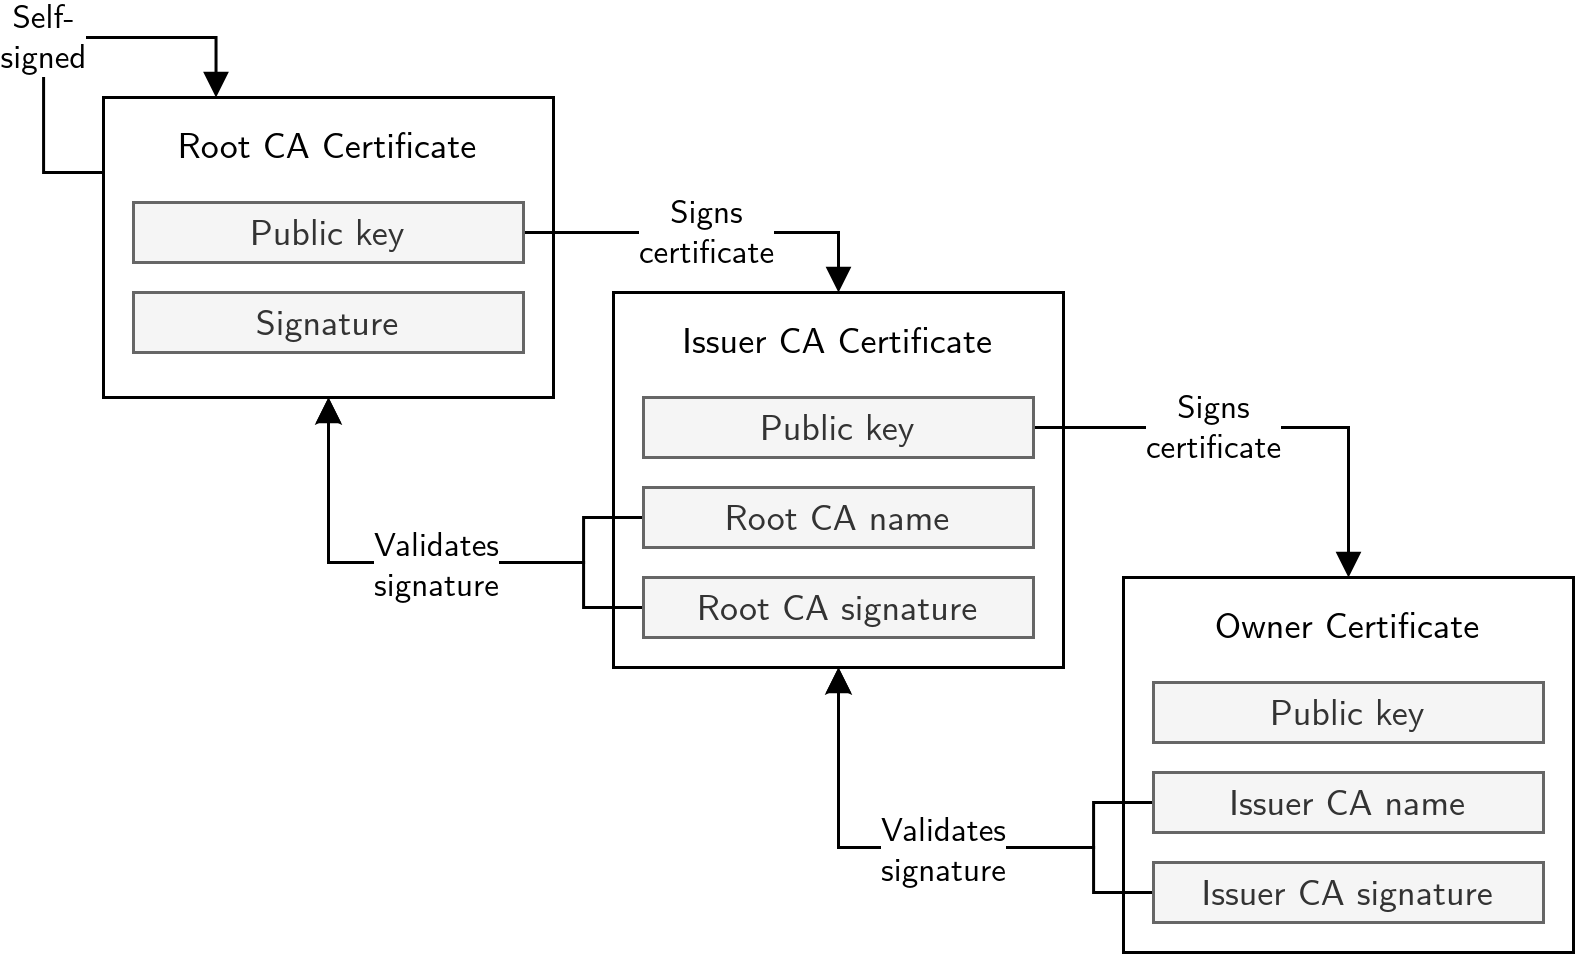
\includegraphics[width=160mm]{images/tls-chain.png}}
\caption[TLS certificate chain of trust]{A chain of trust established between the unknown owner certificate and the implicitly trusted root CA certificate in order to authenticate the identity of the owner against its associated public key.}
\label{tls_chain_figure}
\end{figure}

An organisation or individual must request new certificates from a CA using a Certificate Signing Request (CSR). The CA is then responsible for verifying the identity of the organisation or individual before issuing the certificate. To ensure the validity of certificates are consistent over time, X.509 certificates expire after a set period and must be renewed. Today, this renewal procedure has been widely automated using the Automatic Certificate Management Environment (ACME) protocol, which allows for web servers to complete challenges set by the CA to prove ownership of their domain name and public key without human involvement~\cite{rfc8555}. This has enabled a much shorter certificate rotation period, and it is common to see certificates set to expire within three months.

Through this process, an entity is only required to trust a few well-established root certificates to be capable of validating the authenticity of many certificates and their public keys. These root certificates are generally installed by an inherently trusted party such as the device manufacturer or operating system, but new certificates may be installed by the user.

Typically on the Internet, it is only necessary for the identity of the server be authenticated by the client, while the client remains unauthenticated to the server in the TLS context. In either case, certificates may be exchanged between the server and client during the TLS handshake.

\subsection{TLS 1.3 Handshake}

The TLS handshake is the series of messages exchanged between the client and server to establish the connection. It specifies the steps required to negotiate connection parameters, authenticate peer identities and yield a shared secret. TLS 1.3 was designed to improve the security and performance of the handshake over TLS 1.2 while reducing its overall complexity. Highlighted in these changes is the integration of parameter negotiation into the first client message, enabling encryption of much more of the handshake as well as allowing application data to be sent by the client after only one round trip.

\begin{figure}[ht]
\centerline{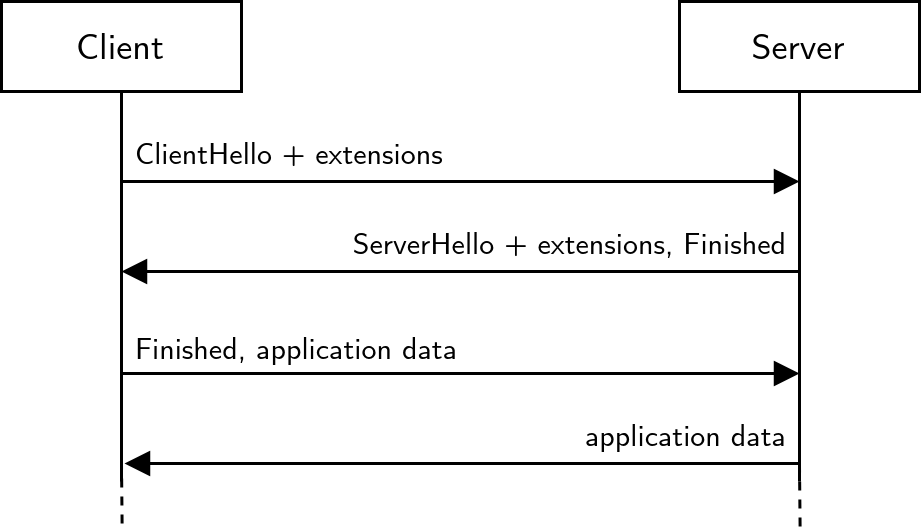
\includegraphics[width=120mm]{images/tls-handshake.png}}
\caption[Basic TLS 1.3 handshake]{Sequence diagram between a client and server describing a basic TLS 1.3 handshake with only server authentication.}
\label{tls_handshake_figure}
\end{figure}

Once a reliable transmission channel has been created between the client and server, a TLS 1.3 handshake can be performed as seen in Fig.~\ref{tls_handshake_figure}. The core functionality of the handshake can be achieved in as few as four message types:

\begin{description}
	\item[ClientHello:] The client initiates the handshake by sending a ClientHello message without any encryption, containing information such as the supported TLS version number, along with a list of available cipher suites and their parameters for the server to choose from. Included in this is also an optimistic key share using the client's preferred cipher suite key exchange method, namely Diffie-Hellman (DH) or Elliptic Curve Diffie-Hellman (ECDH). Both of these generate ephemeral keys for each session, ensuring forward secrecy is preserved in the event the server's private key is compromised. Finally, the ClientHello message also contains a random value generated by the client used to prevent replay attacks.
	\item[ServerHello:] If the server supports the client's preferred cipher suite, it is able to continue the key exchange immediately in the ServerHello message. Otherwise, the server must send a HelloRetryRequest to restart the key share with a different key exchange method which requires an additional round trip. The ServerHello message is sent without encryption and informs the client of what cipher suite and parameters were selected, as well as includes its own random value generated by the server. As the server has now completed its side of the key exchange, all subsequent communication is now encrypted using the selected symmetric encryption algorithm, such as AES-GCM or ChaCha20-Poly1305.
	\item[Certificate:] The server then sends the client its certificate and proof of private key possession by signing a cryptographic hash of the transcript of the handshake so far. It may also choose to request authentication from the client using a CertificateRequest message, which requires the client to respond with its own Certificate message and proof of private key possession.
	\item[Finished:] Finally, the server concludes its side of the handshake by initiating an exchange of Finished messages with the client. This message consists of a Message Authentication Code (MAC) over the cryptographic hash of the transcript of the entire handshake. In this way, the client can confirm success of the key exchange and integrity of the transaction. Once the client has received the ServerHello with the completed key exchange as well as decrypted and validated the Certificate and Finished message, it produces its own Finished message for the server to perform the same checks. Finally, with both peers in agreement on the security of the connection, application data can begin to be securely exchanged.
\end{description}

There are many more complexities to this handshake which are not particularly relevant here that have been omitted from this overview for the sake of brevity. However, one important topic to mention is the inclusion of extensions.

\subsection{Extensions}

Within both the TLS 1.2 and TLS 1.3 handshakes, the ClientHello and ServerHello messages may be extended with additional functionality, which allows the protocol to fulfil a wider range of use cases and accommodate evolving requirements. The usage of extensions has been significantly expanded in TLS 1.3 and now includes the ability for previously unencrypted ServerHello extensions to be placed within the new EncryptedExtensions message sent after ServerHello. Furthermore, a number of new extensions have been defined and several extensions are mandatory to include in the TLS 1.3 handshake. Indeed, the Key Share extension is the provided mechanism for performing key exchanges and the Supported Versions extension is used to signify which versions of TLS is supported.

Nevertheless, the ClientHello message is not encrypted and all of its extensions are sent in the clear. Some of the ClientHello extensions include potentially sensitive information such as the Server Name Indication (SNI) and Application Layer Protocol Negotiation (ALPN) list. It is this privacy weakness that the purposed ECH extension is attempting to remedy.









\section{The Domain Name System}

The Domain Name System (DNS) was designed by Paul Mockapetris in 1984 as a replacement for the manually maintained and shared HOSTS.TXT file used in Internet Protocol (IP) networks to map hostnames to IP addresses, which was becoming increasingly impractical as networks grew in size and complexity~\cite{rfc1034, rfc1035}. Instead, DNS offers a naming system that associates hierarchical alphanumeric identifiers, referred to as domain names, with various resource records, like IP addresses. In this context, a zone is defined as the set containing a domain and all of its subdomains.

Citing significant scalability concerns due to the expected size of the service and the frequency of resource record updates, Mockapetris listed the distributed storage and management of domain name entries with local caching as a design goal for DNS. To address this, the naming system information is distributed as zones amongst many name servers such that each name server is capable of either directly operating on the requested domain name resource records or referring to another name server which is hierarchically closer to the requested domain name. The name server which manages a zone is considered the authoritative name server for the zone. With this, DNS can be used to translate from the more flexible and easily remembered domain names into the associated IP addresses and other resources required to access network applications and services.

\subsection{Name Resolution Process}

A client attempting to resolve a domain name may invoke requests across several name servers. Typically, the client operates as a stub resolver which delegates the task to a known recursive resolver, such as through their network router or Internet service provider (ISP). This is generally done to allow for the caching of DNS query results for use by a whole network or organisation. This situation can be seen in Fig.~\ref{dns_resolve_figure}, where the client has requested the recursive resolver to retrieve resource records for `www.example.com'. To execute the DNS query, the recursive resolver needs to locate the authoritative name server for the requested domain name. Without prior knowledge or cached results, the resolver first queries one of the well-known root name servers to begin navigation of the name hierarchy. In accordance with the distributed nature of DNS, the root name server does not contain the resource records for the requested domain name, but instead directs the resolver to the top-level domain (TLD) name server for `.com'. The resolver reiterates its query to the TLD name server and is again pointed further down the hierarchy, this time to the authoritative name server for `example.com'. Finally, the resolver queries this name server and retrieves the request resource records, which are then returns to the client. All of these results are cached by the recursive resolver for a set amounts of time as specified by the Time To Live (TTL) contained within all responses to help reduce overall load on the system, especially root name servers.

\begin{figure}[ht]
\centerline{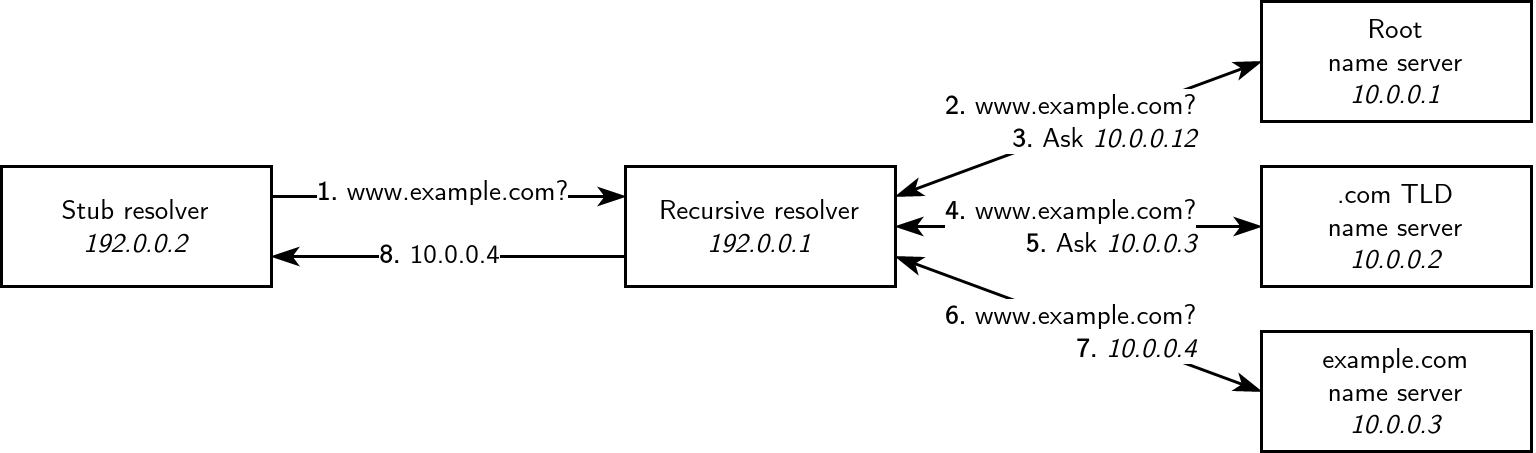
\includegraphics[width=160mm]{images/dns-resolve.png}}
\caption[Example DNS name resolution process]{A stub resolver requests a recursive resolver to retrieve resource records for `www.example.com'. Without previously cached query responses, the recursive resolver must navigate the domain name hierarchy starting at a known root name server.}
\label{dns_resolve_figure}
\end{figure}

\subsection{DNS over HTTPS}

Notably, Mockapetris makes no mention of security nor privacy in the original DNS specification and such concerns have only begun to be addressed in recent years~\cite{rfc7626}. This has largely been due the naming system information being perceived as public knowledge and not requiring security mechanisms. As such, DNS query and response communication have historically been sent unencrypted using the User Datagram Protocol (UDP). It has not been until the last decade with the revelations of widespread global surveillance that issues such as these have started to see much more attention. In 2013, Alissa Cooper et al. wrote extensively on the formulation of privacy threats and mitigations for consideration during the design of Internet protocols, and lists surveillance as being a prevalent privacy threat~\cite{rfc6973}. Following this, Stephen Farrell and Hannes Tschofenig emphasised the danger of exposing protocol content and metadata to large scale surveillance operations and recommends mitigation through security-conscience protocol design~\cite{rfc7258}.

In an effort to apply these learnings, both DNS over TLS (DoT) and DNS over HTTPS (DoH) were conceived as methods for performing privacy-preserving DNS queries~\cite{rfc7858, rfc8484}. Both protocols add confidentiality and data integrity to DNS by encapsulating queries and responses inside secure TLS channels. The most notable difference between the standards is the port number used, as DoT traffic goes to the non-standard port 853 while DoH is served through the standard HTTPS port 443. This difference has lead to some adoption problems with DoT when compared to DoH, as it is not unusual for network firewalls to prohibit traffic to non-standard ports. This also has the effect of making DoT usage being quite conspicuous, while DoH disguises itself amongst other HTTPS traffic. Sebasti{\'a}n Garc{\'\i}a et el. list these as factors when measuring a wider adoption of DoH in 2021~\cite{garcia2021large}.

\subsection{The HTTPS Resource Record}

Today, a number of DNS resource record types exist to fulfil more complex requirements and introduce advanced capabilities. The HTTPS resource record and the more general Service Binding (SVCB) resource record have recently been standardised to allow for specification of additional parameters related to service endpoint discovery and connection establishment~\cite{rfc9460}. This enables more information to be provided to the client needed to access a service while helping to avoid unnecessary round trips and DNS queries. This information set can include items such as the preferable IP address, port number and ALPN list used to connect to a service endpoint which must otherwise be retrieved separately through potentially suboptimal channels.

While ostensibly useful for reducing overall connection latency, the ability for these new resource records to associate parameters with service endpoints facilitates much more flexibility within DNS. In particular, the ECH extension delegates public key and metadata dissemination to this mechanism though the specification of an appropriate `ech` parameter for each service endpoint.








\section{Encrypted Client Hello}

Encrypted Client Hello (ECH) is a proposed extension to TLS 1.3 which has begun to see implementation and adoption on the Internet~\cite{ietf-tls-esni-18, tsiatsikas2022measuring, CF-ECH}. ECH seeks to allow encryption of the ClientHello message, which can contain potentially sensitive information such as the SNI and ALPN extensions. Exposure of the target domain name of the client's request through the SNI was previously considered acceptable due this information being revealed through other channels, but these leaks are becoming less exploitable: Cloud hosting providers, content delivery networks (CDNs) and reverse proxies have diluted the mapping from IP addresses to domain names, the use of encrypted DNS such as DoH is now concealing client DNS queries and the TCP 1.3 handshake encrypts the server certificate. As we have seen in the previous sections, the TLS and DNS ecosystems have adapted to new security and privacy expectations in recent years and are now equipped to support ECH.

The functionality of ECH is based on clients using the public key of an ECH-service provider to send an encrypted TLS 1.3 ClientHello message, which the provider decrypts and uses to proxy the TLS 1.3 connection to the true origin server. The provider must first generate an ECH encryption key pair and some associated metadata. This public key and metadata, referred to as an ECH configuration or ECHConfig, may then be shared out-of-band with ECH-enabled clients though a secure context like DoH using the `ech' parameter in HTTPS resource records. A client may then use this public key and metadata to construct a ClientHello message, named the ClientHelloOuter, holding unremarkable values for the provider alongside the ECH extension containing an encrypted ClientHello, named the ClientHelloInner, itself holding the real values for a private domain. To establish a TLS connection to the origin server of this domain, the client initiates a TLS connection using the ClientHelloOuter with the provider, which decrypts the ClientHelloInner and relays the connection to the origin server, which itself completes the TLS handshake with the client through the provider. Importantly, the provider is incapable of eavesdropping on this secure channel, as the TLS connection is authenticated and end-to-end encrypted between the client and origin server. In this way, the true ClientHello message remains private through the use of public key encryption.

\subsection{Hybrid Public Key Encryption}

ECH uses the Hybrid Public Key Encryption (HPKE) specification for performing public key encryption~\cite{rfc9180}. HPKE defines a standard scheme for combining the use of asymmetric and symmetric cryptographic algorithms such that the performance of symmetric cryptography can be used where only the public key of the receiver is known. This is achieved through using the public key of the receiver to generate a symmetric encryption key as well as an encapsulated shared secret. This encapsulated shared secret can be sent to the receiver which can generate the symmetric encryption key using its private key. Any ciphertext produced by the sender using the symmetric encryption key can now be decrypted by the receiver.

% TODO: cryptography explanation? https://medium.com/asecuritysite-when-bob-met-alice/for-security-go-hybrid-hybrid-public-key-encryption-hpke-1911da1ff831

Furthermore, HPKE provides mechanisms authenticated associated data (AEAD) <aead for ClientHelloOuter>

Karthikeyan Bhargavan, Vincent Cheval, and Christopher Wood have been able to formally verify the security of HPKE in the context of ECH through an automated formal analysis of the privacy properties of the TLS 1.3 handshake~\cite{bhargavan2022symbolic}. <>

\subsection{Split Mode Deployment}

<ech defines two modes of network topology>
<shared mode is when the client-facing server and backend server are co-located, and is not of interest to us>
<split mode is when the client-facing server and backend server are in different boxes pysically separated>
<Fig.~\ref{ech_split_mode_figure}>

\begin{figure}[ht]
\centerline{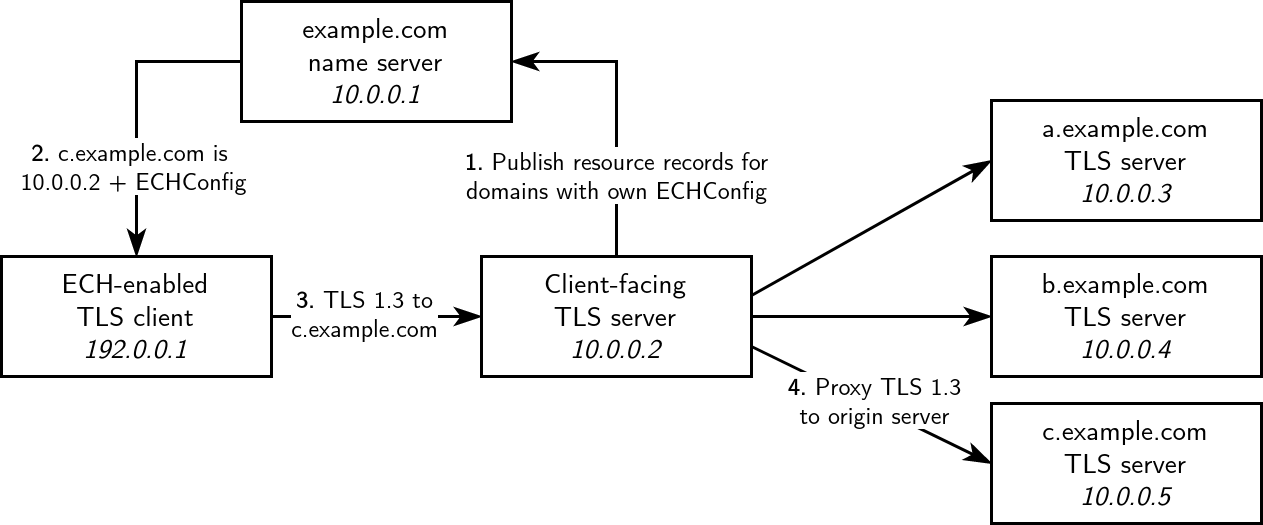
\includegraphics[width=160mm]{images/ech-split-mode.png}}
\caption[Example ECH Split Mode deployment]{<>}
\label{ech_split_mode_figure}
\end{figure}

<this is useful for x,y,z...>
<distributed deployment explanation (as opposed to centralised and decentralised)>
<however it is susceptible to attacks>







\section{Traffic Analysis}

<what is traffic analysis>
<traffic analysis techniques that can be used to infer sensitive information from patterns in network activity>
<exploits information unintentionally leaked by the system aka side-channel attack>
<example of the act of communication being information itself>
<there are a lot of other techniques that can be used: packet inspection>

\subsection{Correlation Attacks}

<is a large category of attacks identified by correlating communication patterns>
<can be used to break anonymity, very relevant to ech split mode>
<examples: timing, packet size, packet count, packet rate+pattern>

\subsection{Countermeasures}

<to disrupt the patterns>
<effectiveness against practicality>
<examples: morphing, mixing/pacing and padding, normalisation>








\section{Summary}

TLS and DNS continue to evolve as their requirements shift in response to modern security and privacy demands. From this movement, the ECH extension for TLS 1.3 has emerged to enable the encryption of the ClientHello message and thereby addressing one of the last points an attacker can learn of potentially sensitive information such as the SNI and ALPN list. The ECH standard defines Split Mode as a network topology which permits the ECH-service provider to be physically separate from the origin server. However, such a situation reveals a potential attack surface against the extension through traffic correlation, which must be disrupted using various practical countermeasures.
